\section{模型}
\label{sec:model}

\subsection{记号与复合结构}
\label{sec:notation}

PBM 作用于 $[0,1]$ 的 sRGB 显示值；不进行线性化、传递函数或颜色空间转换。模型是混色核心与修复层的复合，
\begin{equation}
\mathbf{o}=\clamp\bigl(\mathbf{C}+\mathbf{d},\,0,\,1\bigr),\qquad
\mathbf{C}=\operatorname{Core}(\cb,\ct,\alpha),\qquad
\mathbf{d}=\operatorname{Repair}(\cb,\ct,\alpha,\mathbf{C}),
\label{eq:composition}
\end{equation}
其中 $\cb$ 为基色、$\ct$ 为染色、$\alpha=\clamp(A,0,1)$ 为染色占比：$\alpha=0$ 返回基色，$\alpha=1$ 返回染色。

\begin{figure}[t]
\centering
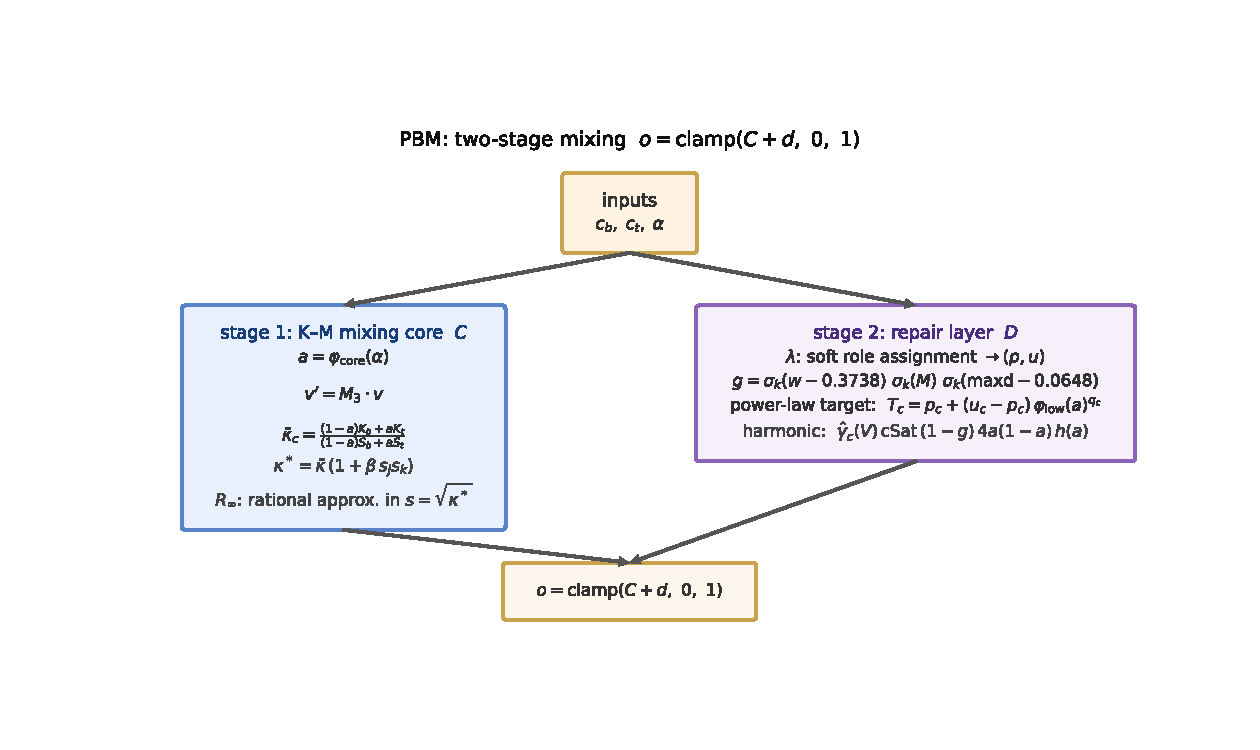
\includegraphics[width=0.82\linewidth]{fig2-architecture.pdf}
\caption{PBM 数据流。两个输入进入 K--M 混色核心（$C$）。修复层分配颜料端与亮端角色（$\lambda$），在门控 $g$ 下计算逐通道幂律目标（$T$），并叠加谐波修正（$\hat{\gamma}$）。修正 $\mathbf{d}$ 加到核心输出后截断。}
\label{fig:architecture}
\end{figure}

修复层对其两个参数的角色是不对称的，而核心是对称的。软角色分配把两种角色次序混合，使完整模型交换对称，
\begin{equation}
F(\cb,\ct,\alpha)\equiv F(\ct,\cb,1-\alpha),
\label{eq:symmetry}
\end{equation}
精确到浮点舍入。

记 $\vp$ 为颜料端、$\vu$ 为亮端（由 \cref{sec:role} 的角色分配选出：最大通道较小的输入扮演颜料）。由 $\vp$ 定义
\begin{equation}
M=\max(\vp),\qquad m=\min(\vp),\qquad \mathrm{maxd}=M-m,\qquad
w=\max\bigl(\min(\vp),\min(\vu)\bigr).
\label{eq:notation}
\end{equation}
斜率为 $k$ 的软阶跃为 $\sigmak(x)=\clamp(kx,0,1)$，$\ssf(x;a,b)$ 表示区间 $[a,b]$ 上的 $C^{1}$ smoothstep。

\subsection{显示值 K/S 混合的结构性缺陷}
\label{sec:defect}

核心在显示值空间中使用解析的吸收与散射默认值进行混合：
\begin{equation}
K(v)=\tfrac12(1-v)^{2},\qquad S(v)=\max(v,\varepsilon),\qquad \varepsilon=0.00157634.
\label{eq:ks-default}
\end{equation}
对白色输入 $v=1$，故 $K=0$、$S=1$；而深色颜料的 $S$ 在 $0.05$--$0.35$ 范围。任意 $\alpha$ 下，白色的散射都主导浓度加权比值的分母，逐通道 $\kappa$ 相互塌缩。

以单通道为例，忽略跨通道矩阵与互吸收修正，考察深蓝 $\#0D1B44=(0.051,0.106,0.267)$ 与白在 $\alpha=0.5$ 时的红通道：
\begin{equation}
\bar{\kappa}_{R}=
\frac{0.5\,K(0.051)+0.5\,K(1)}{0.5\,S(0.051)+0.5\,S(1)}
=\frac{0.5\times0.451}{0.5\times0.051+0.5\times1}=0.429,
\label{eq:defect}
\end{equation}
对应 $\Rinf\approx0.41$。参考 Mixbox 在该通道读出 $0.28$：吸收通道被冲淡。反之蓝通道参考读出 $0.89$，而单通道计算只有 $0.53$：亮化不足。这一失衡是结构性的：白色的 $S=1$ 在任意 $\alpha$ 下都主导混合分母，而加权的 $K$ 与 $S$ 受同一组权重约束，因此在混合阶段重新缩放 $K/S$ 无法恢复被吸收的通道。原始显示值 K--M 叠加在深色加白套件上的平均 $\Delta E_{00}$ 为 10.30（\cref{tab:insample}）。

\subsection{阶段一：K--M 混色核心}
\label{sec:core}

两个输入先经行和为 1 的跨通道矩阵 $\Mthree$ 变换：
\begin{equation}
\mathbf{v}'=\Mthree\mathbf{v},\qquad
\Mthree=
\begin{pmatrix}
0.74523981 & 0.30403013 & -0.04926994\\
0 & 0.74093256 & 0.25906744\\
0 & 0 & 1
\end{pmatrix}.
\label{eq:m3}
\end{equation}
吸收与散射用 \cref{eq:ks-default} 的解析默认值求值。各通道的混合比遵循 Duncan 的浓度结构，并截断到 $[10^{-6},10^{4}]$：
\begin{equation}
\bar{\kappa}_{c}=
\frac{(1-a)\,K(v'_{b,c})+a\,K(v'_{t,c})}
     {(1-a)\,S(v'_{b,c})+a\,S(v'_{t,c})},
\label{eq:kappa}
\end{equation}
其中 $a=\varphi_{\mathrm{core}}(\alpha)$ 为端点压缩后的进度。

逐通道互吸收修正使用另外两个通道 $\{j,k\}$：
\begin{equation}
s'_{c}=\frac{\sqrt{\bar{\kappa}_{c}}}{1+\sqrt{\bar{\kappa}_{c}}},\qquad
\kstar_{c}=\bar{\kappa}_{c}\bigl(1+\beta_{c}\,s'_{j}\,s'_{k}\bigr),\qquad
\beta=(-0.69372345,\,-0.48397409,\,-0.24977842).
\label{eq:beta}
\end{equation}
由于 $s'\in[0,1)$ 且 $\beta_{c}<0$，当其他通道较亮时该修正降低 $\kappa$。

反射率用 $s=\sqrt{\kstar}$ 的有理逼近求值：
\begin{equation}
\Rinf\approx\frac{1}{1+s\bigl(a_{1}+s(a_{2}+s\,a_{3})\bigr)},\qquad
(a_{1},a_{2},a_{3})=\Bigl(\sqrt{2},\,1,\,\tfrac{1}{2\sqrt{2}}\Bigr),
\label{eq:rational}
\end{equation}
该式与 $\Rinf$ 在 $s=0$ 处的前四阶 Taylor 系数一致。在截断范围 $\kstar\in[10^{-6},10^{4}]$ 内，\cref{eq:rational} 的最大绝对误差为 $8.1\times10^{-3}$（在 $\kstar\approx8.1$ 处）；$\kstar\le1$ 时为 $2.5\times10^{-3}$。输出经反变换并截断：
\begin{equation}
\mathbf{C}=\clamp\bigl(\Mthree^{-1}\,\Rinf(\boldsymbol{\kstar}),\,0,\,1\bigr).
\label{eq:core-output}
\end{equation}

\paragraph{动态进度.}
参考在 $\alpha\to1$ 时比显示值 $\kappa$ 混合收敛更快。对 $\alpha=0.99$ 反解参考表明，幂律目标需要的等效进度约为 $10^{-3}$（\cref{sec:inversion}），即 99\% 的混合表现得像 99.9\%。我们用一个作用于核心混合比的对称端点压缩映射来编码这一点：
\begin{equation}
\varphi_{\mathrm{low}}(x)=
\begin{cases}
x, & x\ge w_{\varphi},\\[2pt]
\bigl(1-\ssf(x;0,w_{\varphi})\bigr)x^{p_{\varphi}}+\ssf(x;0,w_{\varphi})\,x, & x<w_{\varphi},
\end{cases}
\label{eq:philow}
\end{equation}
\begin{equation}
\varphi_{\mathrm{core}}(x)=
\begin{cases}
\varphi_{\mathrm{low}}(x), & x<0.5,\\
1-\varphi_{\mathrm{low}}(1-x), & x\ge0.5,
\end{cases}
\label{eq:phicore}
\end{equation}
其中 $p_{\varphi}=1.96522814$、$w_{\varphi}=0.08$。该映射 $C^{1}$ 且关于 $x=0.5$ 反对称，因此核心保持交换对称；当 $x\ge w_{\varphi}$ 时 $\varphi_{\mathrm{low}}(x)=x$，故只影响两端尾部。

\subsection{阶段二：修复层}
\label{sec:repair}

修复层计算加到核心输出上的修正 $\mathbf{d}$，由角色分配、门控、逐通道幂律目标与加性谐波修正组成。

\paragraph{软角色分配.}
\label{sec:role}
颜料端是最大通道较小的输入。硬 argmin 会在 $\max(\cb)=\max(\ct)$ 处不连续切换，故使用软隶属度
\begin{equation}
\lambda=\ssf\!\left(\frac{\max(\ct)-\max(\cb)+E_{W}}{2E_{W}};\,0,\,1\right),
\qquad E_{W}=0.08.
\label{eq:lambda}
\end{equation}
$\lambda=1$ 取 $(\vp,\vu,a)=(\cb,\ct,\alpha)$；$\lambda=0$ 取 $(\ct,\cb,1-\alpha)$；在平局带 $|\max(\ct)-\max(\cb)|<E_{W}$ 内两分支混合：
\begin{equation}
\mathbf{d}=\lambda\,D(\cb,\ct,\alpha)+(1-\lambda)\,D(\ct,\cb,1-\alpha).
\label{eq:dblend}
\end{equation}
带外 $\lambda$ 恰为 $0$ 或 $1$，修复层退化为一次 $D$ 求值。对均匀采样的 sRGB 颜色对，该带约占 $26\%$（在 seed 20260808 的 T3 抽样上实测 26.6\%，在 $2\times10^{5}$ 个均匀对上实测 26.2\%）；因此约四分之三的随机输入会跳过该分支。角色信号取最大通道；也考虑过亮度信号，但它会改变相当比例的随机对的角色判定，故未采用。

\paragraph{深色加亮端门控.}
幂律目标只在深色颜料/亮端区域启用。门控是三个共享斜率 $k=11.0163945$ 的软阶跃之积：
\begin{equation}
g=\sigmak(w-0.37375181)\cdot\sigmak(M)\cdot\sigmak(\mathrm{maxd}-0.06479933).
\label{eq:gate}
\end{equation}
第一个因子在亮端接近消色亮色（$w$ 较大）时开启；第二个在近黑颜料（$M\lesssim1/k\approx0.09$）时压低门控；第三个要求最小色度范围。每个过渡的宽度为 $1/k\approx0.091$，故门控不引入硬截断。对亮色或近消色颜料，$g=0$，直接使用核心输出。

\paragraph{幂律目标.}
在门控区域内，目标遵循从颜料指向亮端的逐通道幂律：
\begin{equation}
T_{c}=p_{c}+(u_{c}-p_{c})\,\varphi_{\mathrm{low}}(a)^{q_{c}}.
\label{eq:target}
\end{equation}
指数 $q_{c}$ 控制通道 $c$ 的亮化速度，由四项组成。

\emph{(a) 软阶跃阶梯.} 在锚点色上反解参考（\cref{sec:inversion}）表明所需指数随通道值 $v$ 下降：暗段保持吸收（高 $q$），亮段快速推进（低 $q$）。该结构由两个阶跃表示：
\begin{equation}
q^{f}(v)=c_{1}^{f}+(c_{2}^{f}-c_{1}^{f})\,\sigmak(v-t_{1})+(c_{3}-c_{2}^{f})\,\sigmak(v-t_{2}),
\qquad f\in\{B,G\},
\label{eq:staircase}
\end{equation}
其中 $t_{1}=0.04350222$、$t_{2}=0.26436295$，系数见 \cref{tab:softstep}。红族为中性，$q^{R}\equiv1$；其通道相关行为由 (d) 的方向响应承担。

\begin{table}[t]
\centering
\small
\caption{亮化指数软阶跃系数（\cref{eq:staircase}）。}
\label{tab:softstep}
\begin{tabular}{lcccc}
\toprule
族 & $c_{1}$（暗） & $c_{2}$（中） & $c_{3}$（亮） & 阶跃位置 / 斜率 \\
\midrule
$B$（蓝，$B$ 最大） & 0.91483121 & 0.32538955 & 0.18785981 & $t_{1}=0.04350222$，$t_{2}=0.26436295$ \\
$G$（绿，$G$ 最大） & 0.57387051 & 0.596528 & 0.18785981 & $k=11.0163945$（共享） \\
$R$（红） & --- & --- & --- & $q^{R}\equiv1$ \\
\bottomrule
\end{tabular}
\end{table}

\emph{(b) 族软混合.} 族权重是颜料通道上的两两支配比较：
\begin{equation}
g_{R}=\tfrac12\,\sigma_{8}(v_{R}-v_{G})+\tfrac12\,\sigma_{8}(v_{R}-v_{B}),
\qquad g_{G}、g_{B}\ \text{同理},
\label{eq:family-weights}
\end{equation}
其中 $\sigma_{8}(x)=\clamp(8x,0,1)$。基础指数为
\begin{equation}
q_{c}^{\mathrm{base}}=\frac{g_{B}q_{c}^{B}+g_{G}q_{c}^{G}+g_{R}q_{c}^{R}}{g_{R}+g_{G}+g_{B}}.
\label{eq:qbase}
\end{equation}
当 $g_{R}+g_{G}+g_{B}<10^{-6}$ 时退化为等权平均，覆盖近灰颜料。

\emph{(c) 通道残差.} 对近零通道，参考曲线依赖通道而非颜料。残差是共享幅度乘以光滑包络：
\begin{equation}
q_{c}\mathrel{+}=\mathrm{RES}_{c}\,e(v_{c}),\qquad
e(v)=
\begin{cases}
A\bigl(1-v/W\bigr)^{2}, & v<W,\\
0, & v\ge W,
\end{cases}
\label{eq:residual}
\end{equation}
其中 $A=0.83421324$、$W=0.14196781$，$\mathrm{RES}=(0,\,-0.24164942,\,-0.24164942)$；红通道残差为零。与分段线性包络不同，\cref{eq:residual} 在 $v=W$ 处 $C^{1}$，且只需三个常数而非八个。

\emph{(d) 通道耦合与方向响应.} 两个通道都高的颜色亮化更慢，且各族的线性方向响应作用在颜料通道上：
\begin{equation}
q_{c}\mathrel{+}=0.42818849\,\sigma_{4.13539205}\Bigl(\max_{i\ne c}v_{i}\Bigr),
\label{eq:coupling}
\end{equation}
\begin{equation}
q_{c}\mathrel{+}=g_{R}\,g^{\mathrm{RTH}}\,\delta^{R}_{c}+g_{B}\,\delta^{B}_{c}+g_{G}\,\delta^{G}_{c},
\qquad
g^{\mathrm{RTH}}=\sigma_{8}(v_{R}-0.21929798),
\label{eq:directional}
\end{equation}
其中
\begin{align}
\delta^{R}&=\bigl[-0.28030789-0.31011215\,v_{R},\nonumber\\
&\qquad 0.33194666-1.19791733\,v_{G},\; -0.45218018+1.71390058\,v_{G}\bigr],\nonumber\\
\delta^{B}&=\bigl[0.40713961,\; -0.08390816+0.76274462\,v_{G},\; 0\bigr],\label{eq:deltas}\\
\delta^{G}&=\bigl[-0.2367074+0.72220875\,v_{R},\; 0,\; -0.30067864+1.03098891\,v_{G}\bigr].\nonumber
\end{align}
范围门 $g^{\mathrm{RTH}}$ 是必要的：线性表达式在 $v_{R}=0.21929798$ 以下改变符号。对两个近黑红 $\#280501$ 与 $\#250903$，在 $\alpha\in[0.1,0.9]$ 上关闭该门会把平均 $\Delta E_{00}$ 从 1.80/2.31 抬到 16.06/13.81（最大值从 2.11/2.66 抬到 18.74/16.45）。

\paragraph{谐波修正.}
在互补色对上反解参考（\cref{sec:inversion}）可看到：混合区间中部的残差呈 $4a(1-a)$ 形状，幅度随输入颜色平滑变化。该修正是在比值特征模板上的线性模型，并在两端衰减：
\begin{equation}
d_{c}\mathrel{+}=\hat{\gamma}_{c}(\vp,\vu)\;\mathrm{cSat}(\vp,\vu)\;(1-g)\;4a(1-a)\;h(a),
\label{eq:harmonic}
\end{equation}
其中
\begin{equation}
\begin{aligned}
h(a)&=\sigma_{14}(0.845-a),\\
\mathrm{cSat}(\vp,\vu)&=\ssf\bigl(\max(\vp)-\min(\vp);0.02,0.15\bigr)\\
&\qquad\cdot\ssf\bigl(\max(\vu)-\min(\vu);0.08,0.30\bigr).
\end{aligned}
\label{eq:csat}
\end{equation}
因子 $(1-g)$ 排除深色加亮端区域。色度衰减 $\mathrm{cSat}$ 在任一端点接近消色轴时把修正压到零。该衰减对连续性很重要：比值特征在零色度附近梯度很大，若去掉 $\mathrm{cSat}$，8 位输入扰动下的最大单步输出变化会从 1.39 升到 2.53 $\Delta E_{00}$（\cref{sec:continuity}）。

幅度是每对颜色计算一次的十七特征模板 $V$ 的线性函数：
\begin{equation}
\hat{\gamma}_{c}(\vp,\vu)=w_{0}^{c}+\sum_{j}w_{j}^{c}\,V_{j},
\label{eq:gamma}
\end{equation}
每通道 17 个系数（共 51 个），由互补族与随机测量的语料上的最小二乘拟合得到（\cref{sec:estimation}）。全部特征都是多项式、通道差值的比值或截断线性式：模板不含三角函数，因此谐波修正只需乘法、加法，以及每个比值一次除法。模板定义见 \cref{tab:features}，系数见 \cref{app:coeff}。与学习的潜表示不同，模板由反解测量手工设计，运行时也不存储任何数据。

\begin{table}[t]
\centering
\scriptsize
\setlength{\tabcolsep}{3pt}
\caption{谐波特征模板（含截距共十七个特征，三通道共用）。全部特征由颜料端 $\vp$ 与亮端 $\vu$ 每对计算一次。}
\label{tab:features}
\begin{tabular}{ll}
\toprule
特征 & 定义 \\
\midrule
截距 & $1$ \\
\texttt{lum} & $0.2126\,p_{R}+0.7152\,p_{G}+0.0722\,p_{B}$ \\
\texttt{lumU} & $0.2126\,u_{R}+0.7152\,u_{G}+0.0722\,u_{B}$ \\
\texttt{pm}、\texttt{pn} & $\max(\vp)$、$\min(\vp)$ \\
\texttt{Mmn} & $\max(\vp)\cdot\min(\vp)$ \\
\texttt{span} & $(\max(\vp)-\min(\vp))(\max(\vu)-\min(\vu))$ \\
\texttt{op} & $1-\tfrac12\bigl[(\max(\vp)-\min(\vp))+(\max(\vu)-\min(\vu))\bigr]$ \\
\texttt{u2} & $u_{B}$ \\
\texttt{dcAbs} & $|u_{R}-p_{R}|$ \\
\texttt{wUcP} & $(u_{R}-u_{B})(p_{B}-p_{R})$ \\
\texttt{dg}、\texttt{ur} & $d_{g}=(p_{G}-p_{B})/\max(M-m,\epsilon)$，$u_{r}=(u_{R}-u_{B})/\max(u_{\max}-u_{\min},\epsilon)$ \\
\texttt{drur}、\texttt{dgug} & $d_{r}u_{r}$、$d_{g}u_{g}$，其中 $d_{r}=(p_{R}-p_{B})/\cdots$、$u_{g}=(u_{G}-u_{B})/\cdots$ \\
\texttt{dcmucm} & $d_{cm}u_{cm}$，其中 $d_{cm}=(p_{R}-p_{G})/\cdots$、$u_{cm}=(u_{R}-u_{G})/\cdots$ \\
\texttt{gRu} & $\tfrac12\sigma_{8}(u_{R}-u_{G})+\tfrac12\sigma_{8}(u_{R}-u_{B})$ \\
\bottomrule
\end{tabular}
\end{table}

\subsection{算法与边界行为}
\label{sec:algorithm}

完整流程见 \cref{alg:pbm}。端点复制步骤按构造使 $\alpha=0$ 与 $\alpha=1$ 精确。其余运算都是连续函数的复合——截断、幂、smoothstep 与线性式——因此模型连续；没有任何分支会让输出值不连续跳变。\Cref{tab:boundary} 汇总边界性质与实测值。

其中 $\operatorname{Core}$ 表示 \cref{eq:phicore,eq:m3,eq:kappa,eq:beta,eq:core-output} 的复合，$D$ 表示 \cref{eq:gate,eq:target,eq:harmonic} 的修复分支。

\begin{algorithm}[t]
\caption{PBM 混色.}
\label{alg:pbm}
\KwIn{基色 $\cb$、染色 $\ct$（$[0,1]$ 的 sRGB 显示值），比例 $A$}
\KwOut{混合色 $\mathbf{o}$}
$\alpha\gets\clamp(A,0,1)$\;
\If{$\alpha=0$}{\Return{$\cb$}}
\If{$\alpha=1$}{\Return{$\ct$}}
$\mathbf{C}\gets\operatorname{Core}(\cb,\ct,\alpha)$\;
$t_{e}\gets\clamp\bigl((\max(\ct)-\max(\cb)+E_{W})/(2E_{W}),0,1\bigr)$\;
\uIf{$t_{e}\le0$}{$\mathbf{d}\gets D(\ct,\cb,1-\alpha,\mathbf{C})$}
\uElseIf{$t_{e}\ge1$}{$\mathbf{d}\gets D(\cb,\ct,\alpha,\mathbf{C})$}
\Else{$\lambda\gets\ssf(t_{e})$;\; $\mathbf{d}\gets\lambda D(\cb,\ct,\alpha,\mathbf{C})+(1-\lambda)D(\ct,\cb,1-\alpha,\mathbf{C})$}
\Return{$\clamp(\mathbf{C}+\mathbf{d},0,1)$}\;
\end{algorithm}

\begin{table}[t]
\centering
\small
\caption{PBM 的边界行为。}
\label{tab:boundary}
\begin{tabular}{p{0.28\linewidth}p{0.64\linewidth}}
\toprule
性质 & 保证 \\
\midrule
$\alpha=0,1$ & 精确返回输入（T4 最大通道误差 0.00000）。 \\
门控之外 & $g=0$：核心输出加谐波修正；门控之内：幂律目标加谐波修正；过渡连续。 \\
连续性 & 连续函数的复合；8 位扰动下实测最大单步 $\Delta E_{00}$ 为 1.388，超过 1.53 的次数为零。 \\
交换对称 & $F(\cb,\ct,\alpha)\equiv F(\ct,\cb,1-\alpha)$；在 5000 个随机对上实测最大 RGB 差 $6.7\times10^{-16}$（seed 20260808）。 \\
\bottomrule
\end{tabular}
\end{table}

\paragraph{复杂度与实现.}
模型执行固定数量的算术运算：两个输入矩阵—向量乘、一个输出矩阵—向量乘、六次平方根、至多五次幂运算，且不含三角函数与对数。它没有数据循环、查找表或迭代，时间与空间复杂度为 $O(1)$。参考实现提供四种语言（JavaScript、Python、Java、C++），常数完全一致；对 2000 个随机对的跨语言测试测得最大 RGB 通道差为 $5\times10^{-10}$，与测试使用的九位小数序列化及初等函数的库级差异一致。

模型的常数在实现中冻结。修改它们需要重跑估计流程与跨语言一致性测试；四个端口在数值字面量层面保持一致。
